\section{Experiments}
\label{sec:experiments}

\paragraph{Protocol.}
We use \exdbn's benchmark: \exdbn's generator, parameter grid and evaluation code, called
through a thin bridge. There are three configurations. ER3-p1 has an Erd\H{o}s--R\'enyi
intra-slice graph with $3d$ edges and one lag. SF3-p1 is the same with a scale-free graph.
ER2-p2 has $2d$ edges and two lags. We use $d\in\{5,10,15,20,25\}$, $n\in\{250,1000\}$ and
seeds 0--4, which gives 110 instances (\cref{app:details}). \exdbn{} runs with its own
settings and the 120\,s time limit of its main experiments, on pooled data. By
\cref{prop:gram} this is equivalent to a federated \exdbn{} with secure aggregation.
\feddbn{} splits each series into $K\in\{1,2,4,8\}$ contiguous windows, one per client.
Hyperparameters were fixed beforehand on disjoint tuning seeds. We report SHD and F1 at the
SHD-optimal threshold, as \exdbn{} does.

\subsection{Statistical performance on the \exdbn{} benchmark}
\label{sec:exp-accuracy}

\begin{table}[t]
\centering
\caption{\exdbn{} benchmark: mean over seeds (5, or 4 where \exdbn's generator gave up). \exdbn{}
on pooled data (SHD, F1, final MIP gap after 120\,s) against \feddbn{} with $K$ clients
($K=1$ is centralised \psidbn). ``edges'' is the number of true edges in $W$ and $A$.}
\label{tab:main}
\small
\begin{tabular}{llr rrr rrrrr r}
\toprule
 & & & \multicolumn{3}{c}{\exdbn{} (pooled, 120\,s)} & \multicolumn{5}{c}{SHD of \feddbn{} with $K$ clients} & \\
\cmidrule(lr){4-6}\cmidrule(lr){7-11}
config & $d$ & $n$ & SHD & F1 & gap & $K{=}1$ & 2 & 4 & 8 & F1$_{K=8}$ & edges \\
\midrule
ER3-p1 & 10 & 250 & 4.1 & 0.95 & 0.25 & 15.9 & 17.2 & 17.9 & 17.5 & 0.75 & 48 \\
 & 10 & 1000 & 0.0 & 1.00 & 0.15 & 13.2 & 11.5 & 11.5 & 12.2 & 0.79 & 47 \\
 & 15 & 250 & 14.6 & 0.88 & 0.57 & 35.7 & 34.8 & 32.9 & 34.9 & 0.66 & 71 \\
 & 15 & 1000 & 0.0 & 1.00 & 0.56 & 24.8 & 25.1 & 24.5 & 22.9 & 0.79 & 73 \\
 & 20 & 250 & 50.8 & 0.62 & 0.74 & 57.7 & 57.6 & 57.3 & 59.5 & 0.55 & 93 \\
 & 20 & 1000 & 48.0 & 0.72 & 0.74 & 35.9 & 35.6 & 35.2 & 38.5 & 0.75 & 95 \\
 & 25 & 250 & 93.0 & 0.43 & 0.88 & 74.7 & 74.6 & 74.1 & 75.9 & 0.59 & 119 \\
 & 25 & 1000 & 85.9 & 0.47 & 0.85 & 41.8 & 42.5 & 42.0 & 45.9 & 0.79 & 120 \\
\midrule
SF3-p1 & 5 & 250 & 1.9 & 0.90 & 0.00 & 4.0 & 3.9 & 4.3 & 4.8 & 0.71 & 18 \\
 & 5 & 1000 & 0.2 & 1.00 & 0.00 & 3.8 & 3.8 & 3.8 & 3.8 & 0.78 & 18 \\
 & 10 & 250 & 2.4 & 0.97 & 0.05 & 15.3 & 15.4 & 16.7 & 17.6 & 0.73 & 44 \\
 & 10 & 1000 & 0.0 & 1.00 & 0.03 & 9.7 & 9.5 & 9.1 & 9.0 & 0.87 & 45 \\
 & 15 & 250 & 8.0 & 0.93 & 0.53 & 34.4 & 33.7 & 31.2 & 35.9 & 0.63 & 67 \\
 & 15 & 1000 & 1.7 & 0.99 & 0.41 & 36.8 & 36.9 & 37.1 & 37.3 & 0.65 & 69 \\
 & 20 & 250 & 47.0 & 0.61 & 0.80 & 53.7 & 53.1 & 54.4 & 57.9 & 0.57 & 92 \\
 & 20 & 1000 & 4.4 & 0.97 & 0.66 & 35.8 & 33.6 & 34.4 & 37.0 & 0.77 & 93 \\
 & 25 & 250 & 58.9 & 0.64 & 0.84 & 58.8 & 59.7 & 61.9 & 69.7 & 0.57 & 111 \\
 & 25 & 1000 & 65.2 & 0.63 & 0.84 & 57.5 & 60.8 & 60.2 & 59.1 & 0.67 & 114 \\
\midrule
ER2-p2 & 5 & 250 & 1.0 & 0.97 & 0.00 & 3.9 & 4.1 & 4.9 & 5.3 & 0.83 & 28 \\
 & 5 & 1000 & 0.0 & 1.00 & 0.00 & 2.7 & 2.6 & 2.6 & 3.0 & 0.91 & 28 \\
 & 10 & 250 & 3.0 & 0.97 & 0.28 & 19.4 & 18.0 & 20.8 & 22.9 & 0.70 & 54 \\
 & 10 & 1000 & 0.0 & 1.00 & 0.22 & 6.3 & 6.5 & 7.1 & 7.7 & 0.91 & 55 \\
 & 15 & 1000 & 0.0 & 1.00 & 0.42 & 21.0 & 21.0 & 20.0 & 35.5 & 0.79 & 87 \\
\bottomrule
\end{tabular}

\end{table}

\Cref{tab:main} gives the main comparison. Two regimes stand out.

\emph{Small problems, $d\le 15$ (71 instances).} \exdbn{} is essentially exact: mean SHD
2.6 and F1 0.97, and SHD 0 on most instances with $n=1000$. \feddbn{} is clearly worse, with
mean SHD 16.2 and F1 0.78 for $K=1$, and 17.0 and 0.77 for $K=8$. The relative price of
federation is 27\% of the true edges. This is the price one pays for replacing exact
optimisation by a first-order method with a greedy projection.

\emph{Larger problems, $d\in\{20,25\}$ (39 instances).} With 120\,s and two threads the MIP
is far from optimal: the mean final gap is 0.74 to 0.88. Its SHD jumps to 48--93 on ER3-p1.
Under this budget \feddbn{} matches or beats it: mean SHD 55.7 for $K=8$ against 55.9 for
\exdbn{}, with lower SHD on 18 of the 39 instances. On ER3-p1 with $n=1000$ the difference
is large: 35.9 against 48.0 at $d=20$, and 41.8 against 85.9 at $d=25$. \exdbn{} needs
120--240\,s per instance, of which up to 116\,s is spent building the model. \feddbn{} needs
0.6\,s ($K=1$) to 1.0\,s ($K=8$) of parallel time, two orders of magnitude less.

This crossover depends on the MIP budget. On four of these instances (ER3-p1 and SF3-p1,
$d\in\{20,25\}$, $n=1000$, seed 1) we reran the Gram form of \exdbn{}
(\cref{tab:budget}). With the same budget, 120\,s and two threads, it is as inaccurate as
the original formulation. With 300\,s and six threads, about $7.5\times$ the core-seconds,
it returns the \emph{true} graph (SHD 0) on all four. Its gap, however, stays at 0.50--0.62:
the solver finds the optimum but cannot certify it, as the weak root relaxation of
\cref{sec:mip} predicts. Against an adequately resourced MIP, the price of federation at
$d=20$--$25$ is therefore not negative. It is close to \feddbn's full SHD, about 53\% of the
true edges on average for $K=8$. The honest summary is that \feddbn{} trades this accuracy for a two to three
orders of magnitude smaller and \emph{predictable} compute budget. In both regimes
federation itself is cheap: going from $K=1$ to $K=8$ costs 0.8 SHD on average for $d\le15$
and 3.5 for $d\ge 20$.

\begin{table}[t]
\centering
\caption{Sensitivity of \exdbn{} to its compute budget on four instances with $n=1000$,
seed 1. Original formulation from \cref{tab:main}; Gram form of \cref{prop:gram}.}
\label{tab:budget}
\small
\begin{tabular}{l rr rr rr r}
\toprule
 & \multicolumn{2}{c}{original, 120\,s, 2 thr.} & \multicolumn{2}{c}{Gram, 120\,s, 2 thr.} & \multicolumn{2}{c}{Gram, 300\,s, 6 thr.} & \feddbn{} \\
\cmidrule(lr){2-3}\cmidrule(lr){4-5}\cmidrule(lr){6-7}\cmidrule(lr){8-8}
instance & SHD & gap & SHD & gap & SHD & gap & SHD ($K{=}8$) \\
\midrule
ER3-p1, $d=20$ & 49.0 & 0.79 & 47.5 & 0.89 & 0.0 & 0.53 & 78.5 \\
ER3-p1, $d=25$ & 59.5 & 0.79 & 61.0 & 0.77 & 0.0 & 0.51 & 26.5 \\
SF3-p1, $d=20$ & 0.0 & 0.72 & 0.0 & 0.73 & 0.0 & 0.50 & 49.0 \\
SF3-p1, $d=25$ & 74.0 & 0.84 & 90.0 & 0.88 & 0.0 & 0.62 & 59.5 \\
\bottomrule
\end{tabular}

\end{table}

\subsection{Where does the price come from?}
\label{sec:exp-decomp}

\begin{table}[t]
\centering
\caption{Decomposition \eqref{eq:decomp} of the price of federation with $K=8$ clients,
averaged over the instances of each row. A negative $\Delta_{\mathrm{est}}$ means that least
squares with the true order beats the time-limited MIP.}
\label{tab:decomp}
\small
\begin{tabular}{llr r rrrr r r}
\toprule
config & $d$ & inst. & SHD$_{\mathrm{MIP}}$ & $\Delta_{\mathrm{est}}$ & $\Delta_{\mathrm{order}}$ & $\Delta_{\mathrm{opt}}$ & $\Delta_{\mathrm{fed}}(8)$ & PoF$(8)$ & PoF/edges \\
\midrule
ER3-p1 & 10 & 10 & 2.0 & 3.5 & 9.1 & -0.1 & 0.3 & 12.8 & 27\% \\
 & 15 & 10 & 7.3 & 4.1 & 19.1 & -0.2 & -1.4 & 21.6 & 30\% \\
 & 20 & 10 & 49.4 & -32.9 & 27.5 & 2.8 & 2.2 & -0.4 & 1\% \\
 & 25 & 9 & 89.8 & -62.1 & 31.8 & 0.5 & 2.5 & -27.3 & -23\% \\
\midrule
SF3-p1 & 5 & 10 & 1.1 & -0.4 & 3.2 & 0.0 & 0.4 & 3.2 & 18\% \\
 & 10 & 10 & 1.2 & 1.9 & 9.6 & -0.1 & 0.8 & 12.1 & 27\% \\
 & 15 & 10 & 4.8 & 3.9 & 27.4 & -0.6 & 1.0 & 31.8 & 46\% \\
 & 20 & 10 & 25.7 & -9.9 & 29.1 & -0.1 & 2.7 & 21.8 & 24\% \\
 & 25 & 10 & 62.0 & -39.4 & 36.9 & -1.4 & 6.2 & 2.4 & 3\% \\
\midrule
ER2-p2 & 5 & 10 & 0.5 & 0.1 & 2.6 & 0.1 & 0.8 & 3.6 & 13\% \\
 & 10 & 10 & 1.5 & 3.2 & 8.1 & 0.1 & 2.5 & 13.8 & 25\% \\
 & 15 & 1 & 0.0 & 4.0 & 17.0 & 0.0 & 14.5 & 35.5 & 41\% \\
\midrule
all & & 110 & 21.5 & -11.0 & 18.4 & 0.1 & 1.8 & 9.2 & 18\% \\
\bottomrule
\end{tabular}

\end{table}

\Cref{tab:decomp} decomposes the price of federation. Averaged over all 110 instances,
$\mathrm{PoF}(8)=9.2$ SHD (18\% of the true edges). The terms are as follows.

\textbf{The projection's order is the dominant cost.} $\Delta_{\mathrm{order}}=18.4$ is
twice the total price and grows with $d$, from 2.6--3.2 at $d=5$ to 32--37 at $d=25$. With
the \emph{true} order, exact least squares followed by thresholding is nearly perfect: SHD 3.6
and F1 0.98 for $n=1000$. With the order returned by \psidag's greedy projection, the same
estimator reaches only SHD 23.9. The iteration also rarely revises its first order: on
average only 2.2 distinct orders are visited over 30 epochs.

\textbf{Incomplete optimisation costs almost nothing in the centralised setting.}
$\Delta_{\mathrm{opt}}=0.1$ on average and $|\Delta_{\mathrm{opt}}|\le 2.8$ in every row, so
once the order is fixed, 390 rounds of local accelerated steps solve the convex subproblem to
statistical accuracy. With federation the optimisation error reappears where clients hold
very few samples. For $n=250$ and $K=8$, each client sees 31 time points against up to $m=50$
regressors, and the local problems are underdetermined. The optimisation error of \feddbn{},
SHD relative to the exact refit on its own order, rises from 0.0 ($K=1$) to 4.4 ($K=8$). For
$n=1000$ it rises from 0.1 to 1.1.

\textbf{Federation does not degrade the order.} Averaged over the instances, the federation
term is $\Delta_{\mathrm{fed}}(2)=-0.1$, $\Delta_{\mathrm{fed}}(4)=0.1$ and
$\Delta_{\mathrm{fed}}(8)=1.8$. Its order component,
$\shd(\mathrm{LS}(\hat\pi_K))-\shd(\mathrm{LS}(\hat\pi_1))$, is \emph{negative} for every
$K$ ($-0.4$, $-0.9$, $-0.9$). Averaging local models apparently perturbs the iterate in a
way that helps the greedy projection slightly. The federation cost is therefore entirely
client drift on small local samples, and it shrinks with $n/K$: $\Delta_{\mathrm{fed}}(8)$
is 2.6 for $n=250$ and 0.9 for $n=1000$.

\textbf{The estimator term changes sign with $d$.} For $d\le 15$, $\Delta_{\mathrm{est}}$ is
small and positive (at most 4.1): even with the correct order, thresholded least squares is
slightly worse than the $\ell_0$-penalised MIQP: by 3.6 SHD at $n=250$ and 1.1 at $n=1000$. For $d\ge 20$ it is large
and negative ($-62$ on ER3-p1, $d=25$), because the time-limited MIP is far from its optimum.
That is where \feddbn{} recovers its whole price.

\subsection{Communication: rounds, latency and staleness}
\label{sec:exp-comm}

\begin{figure}[t]
\centering
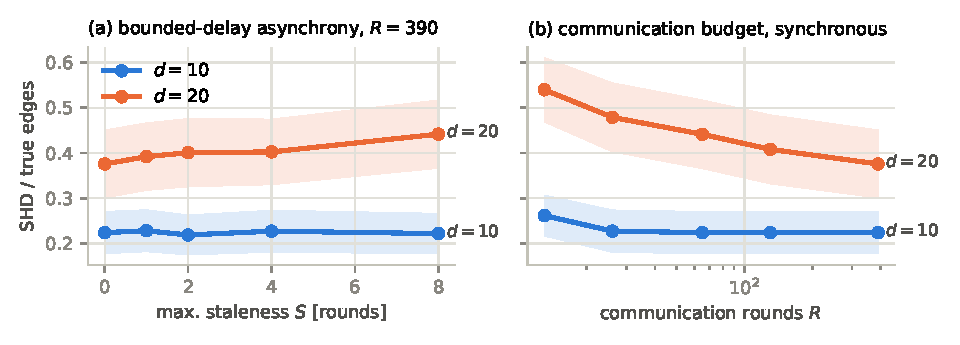
\includegraphics[width=\linewidth]{figures/delay}
\caption{Effect of communication on accuracy ($K=4$ clients, ER3-p1 and SF3-p1, $n=1000$,
mean $\pm$ s.e.m.\ over 10 instances per $d$). (a)~Bounded-delay asynchrony: each client
starts from a model up to $S$ rounds old. (b)~Synchronous \feddbn{} with a budget of
$R$ communication rounds, obtained by varying the number of epochs.}
\label{fig:delay}
\end{figure}

\begin{table}[t]
\centering
\caption{Wall-clock time model \eqref{eq:wallclock} [s]: measured parallel compute time plus
$R(2\ell+16md/\beta)$ for networks with (latency $\ell$, bandwidth $\beta$) = datacentre
(0.1\,ms, 10\,Gb/s), LAN (1\,ms, 1\,Gb/s), WAN (50\,ms, 100\,Mb/s) and cross-continent
(150\,ms, 20\,Mb/s).}
\label{tab:comm}
\small
\begin{tabular}{l r r rrrr}
\toprule
instance & rounds & compute [s] & datacentre & LAN & WAN & cross-continent \\
\midrule
ExDBN bench., $d{=}25$, $K{=}8$ & 390 & 1.0 & 1.1 & 1.9 & 40.7 & 121.1 \\
scaling, $d{=}100$, $K{=}8$ & 130 & 0.9 & 1.0 & 1.5 & 17.2 & 56.6 \\
scaling, $d{=}1000$, $K{=}8$ & 130 & 111.1 & 114.4 & 144.6 & 456.9 & 1814.1 \\
\bottomrule
\end{tabular}

\end{table}

\Cref{fig:delay}(b) shows that the number of rounds matters more than delays. On $d=20$,
13 rounds (one epoch) give a 40--50\% higher SHD than 390 rounds. On $d=10$, 26
rounds already suffice. Bounded staleness, panel (a), is harmless at $d=10$. At $d=20$ it costs
up to 11 SHD on ER3-p1 ($S=8$) but little on SF3-p1. For small models latency dominates the communication cost
(\cref{tab:comm}). On the \exdbn{} benchmark a WAN deployment adds about 40\,s to about one
second of computation. That is still less than the 120\,s the MIP spends in branch-and-bound,
which does not even include gathering the Gram matrix. For $d=1000$ a message has
$md=2\cdot 10^6$ floats (16\,MB), and on slow links bandwidth dominates. A cross-continent
deployment would spend 30 minutes communicating in 130 rounds, so compressing or
sparsifying the updates matters at this scale. In every setting the number of rounds,
not the delay per round, is the quantity to economise.

\subsection{Scalability}
\label{sec:exp-scaling}

\exdbn's generator does not produce instances beyond $d\approx 25$ (\cref{app:details}), so
for scaling we use our own generator for the same model class. It draws an ER intra-slice DAG
with expected degree 4 and one lag with $d$ entries, which gives about $3d$ true edges, with
$n=\max(1000,4d)$, $d$ from 10 to 1000 and three seeds. \feddbn{} runs 130 rounds (10
epochs of 20 local steps). \exdbn{} runs in the Gram form with 120\,s and four threads for
$d\le 250$, and in its original formulation for $d\le 25$ (and for $d=50$ on seed 0, run
alone). \Cref{fig:scaling,tab:scaling}
give the results.

\begin{figure}[t]
\centering
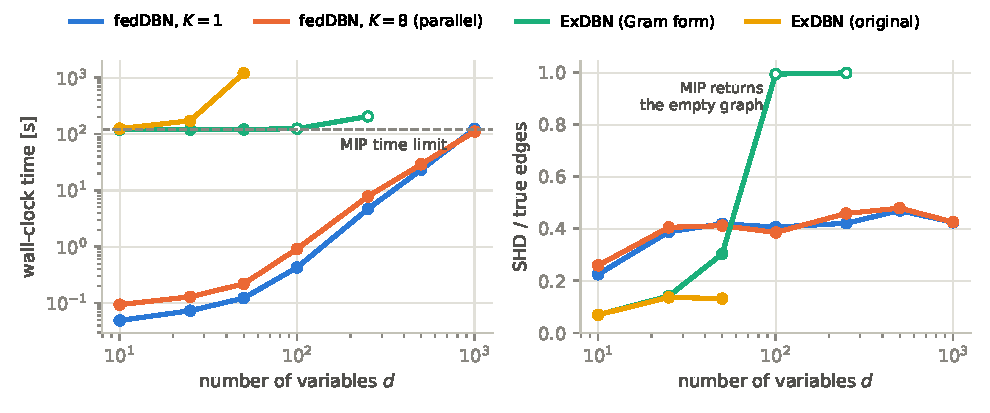
\includegraphics[width=\linewidth]{figures/scaling}
\caption{Scaling on ER instances with one lag and $n=\max(1000,4d)$, mean over three seeds
(one seed for $K=8$ at $d=1000$ and for the original \exdbn{} formulation at $d=50$). Left: wall-clock time. For \feddbn{} this is the parallel
time; for \exdbn{} it is the total time including model building, with the 120\,s limit
dashed. Right: SHD relative to the number of true edges. Hollow markers: the MIP returned the
empty graph.}
\label{fig:scaling}
\end{figure}

\begin{table}[t]
\centering
\caption{Scaling, mean over three seeds (one for $K=8$ at $d=1000$). ``edges'' counts the
true edges in $W$ and $A$. \feddbn{} times are parallel times. \exdbn{} in the Gram form has
a 120\,s limit and four threads. A gap $\gg1$ means that the dual bound is still the trivial
one implied by $|w|\le M$. ``build'' is the time to construct the Gram-form model, and
``orig.'' is the original formulation, with its total time including model building.
$^\dagger$Seed 0 only.}
\label{tab:scaling}
\small
\setlength{\tabcolsep}{4pt}
\begin{tabular}{rr rrr rrr rrrr rr}
\toprule
 & & \multicolumn{3}{c}{\feddbn, $K{=}1$} & \multicolumn{3}{c}{\feddbn, $K{=}8$} & \multicolumn{4}{c}{\exdbn{}, Gram form} & \multicolumn{2}{c}{\exdbn{}, orig.} \\
\cmidrule(lr){3-5}\cmidrule(lr){6-8}\cmidrule(lr){9-12}\cmidrule(lr){13-14}
$d$ & edges & SHD & F1 & time [s] & SHD & F1 & time [s] & SHD & F1 & gap & build [s] & SHD & time [s] \\
\midrule
10 & 30 & 7.2 & 0.79 & 0.05 & 8.5 & 0.78 & 0.09 & 2.3 & 0.96 & 0.01 & 0.02 & 2.3 & 125 \\
25 & 75 & 29.3 & 0.73 & 0.07 & 30.7 & 0.72 & 0.13 & 10.5 & 0.91 & 0.29 & 0.25 & 10.2 & 173 \\
50 & 153 & 64.3 & 0.70 & 0.12 & 63.2 & 0.71 & 0.22 & 46.3 & 0.78 & 0.39 & 0.81 & 20.0$^\dagger$ & 1205$^\dagger$ \\
100 & 303 & 124.0 & 0.73 & 0.43 & 117.8 & 0.75 & 0.92 & 301.7 & 0.00 & $\gg 1$ & 4.80 & -- & -- \\
250 & 771 & 324.5 & 0.73 & 4.65 & 354.2 & 0.72 & 7.80 & 770.0 & 0.00 & $\gg 1$ & 85 & -- & -- \\
500 & 1500 & 705.0 & 0.71 & 23 & 719.0 & 0.67 & 29 & \multicolumn{4}{c}{not attempted} & -- & -- \\
1000 & 2983 & 1267.3 & 0.75 & 124 & 1282.5 & 0.76 & 111 & \multicolumn{4}{c}{not attempted} & -- & -- \\
\bottomrule
\end{tabular}

\end{table}

\textbf{\feddbn's accuracy does not degrade with $d$.} From $d=25$ to $d=1000$ its SHD
stays between 0.39 and 0.48 of the true edges and its F1 between 0.67 and 0.76, for both $K=1$
and $K=8$. Federation costs little at every size: the relative SHD of $K=8$ and $K=1$
differs by at most 0.04.

\textbf{\feddbn's running time is polynomial and predictable.} It grows from 0.05\,s at
$d=10$ to 124\,s at $d=1000$ for $K=1$. A local step multiplies the $m\times m$ Gram matrix
by the $m\times d$ iterate, which costs $O(d^3)$ flops. The measured time grows as
$d^{2.4}$ between $d=250$ and $d=1000$. For $K=8$ at $d=1000$ the parallel time is 111\,s
and the sequential time 761\,s. Each client's local step costs as much as a centralised step,
whatever $n_k$, because it uses an $m\times m$ Gram matrix. Federation therefore brings data
locality, not a speed-up. For $d\le 250$ the parallel time of $K=8$ is 1.7--2.1 times that
of $K=1$, partly because each round waits for the slowest of eight clients.

\textbf{The MIP stops returning useful graphs at $d=100$.} Up to $d=50$, \exdbn{} is clearly
more accurate than \feddbn: its relative SHD is 0.07, 0.14 and 0.30, against 0.23, 0.39 and
0.42 for \feddbn{} with $K=1$. Over the same range its gap grows from 0.01 to 0.39. At
$d=100$ (19\,900 binaries) it returns exactly the empty graph on all three seeds. Its
incumbent is $\Theta=0$, with objective $\operatorname{tr}(S_{XX})$, and its dual bound is
$-8\cdot10^{9}$. On seed 0, Gurobi's log shows that the \emph{root relaxation} hit the time
limit after $6.8\cdot10^4$ simplex iterations in a 45\,s run, and the 120\,s run ends with the
same bound. This convex
QP has $4\cdot10^4$ variables and $2\cdot10^6$ quadratic terms, and the sequential solver
does not solve even this one node. That is the bottleneck of \cref{sec:mip}, reason~3, in its
plainest form. At $d=250$ building the Gram-form model alone takes 85\,s, and the result is
again the empty graph. Within this budget the crossover therefore lies between $d=50$ and
$d=100$. Beyond it, \feddbn{} is the only one of the two methods that returns a graph, with
SHD about 0.4 of the true edges.

\textbf{The original formulation is limited by model building.} It is as accurate as the
Gram form at $d\le 25$ (relative SHD 0.07 and 0.14), but its total time is 125\,s at $d=10$
and 173\,s at $d=25$. That is about 50\,s of model construction on top of the time limit, and the
number of terms to construct grows as $n d m^2$ (\cref{sec:mip}). At $d=50$ (seed 0) the
build takes about 1085\,s, eighteen minutes, and peaks at 12.3\,GB of memory. In its 120\,s
of branch-and-bound this run then found a much better graph than the Gram form on the same
instance: SHD 20 and F1 0.92, against 56 and 0.72, with a similar gap (0.35 against 0.39).
\feddbn{} reaches 60.5 ($K=1$) and 62 ($K=8$) on this instance. The two formulations define the
same optimisation problem, so the difference reflects how sensitive a time-limited
branch-and-bound is to presolve and search order, and to the fact that this run had the
machine to itself. One instance is not enough to say more. It does show that the ranking up
to $d=50$ favours the MIP, \emph{if} one can afford to build the model.
